\documentclass[14pt]{beamer}
\usetheme{Warsaw}
\usecolortheme{beaver}
\usefonttheme{professionalfonts}

\input{../../preamble}
\usepackage{amscd,amsmath,amssymb,amsthm,graphicx}
\usepackage{paralist}
\usepackage{tabto}
\usepackage[normalem]{ulem}
\usepackage{tikz}
\usepackage{tkz-euclide}
\usetkzobj{all}
\newcommand{\dint}{\displaystyle\int}
\newcommand{\dlim}{\displaystyle\lim}
\newcommand{\dsum}{\displaystyle\sum}

% % % % % % % % % %
\title[Cal I S2015]{MATH 2554 (Calculus I)}
\subtitle{}
\author[Wheeler]{Dr. Ashley K. Wheeler}
\institute{University of Arkansas}
\date{\today}
\logo{}

% % %
\begin{document}
\maketitle

% % %
\begin{frame}
\frametitle{Table of Contents}
\tableofcontents
\end{frame}

% % % % % % % % % % Mon 6 Apr 2015

% % %
\begin{frame}
\section[Week 12]{Week 12: 6-10 April}
\frametitle{Monday 6 April (Week 12)}
\small
\begin{itemize}
\item Exam \#3: Is now a Take Home.  Returned in drill tomorrow.  Due Friday in class.
\item Computer HW this week: $\oint 4.6-4.7$ 	
\item Quiz \#11 Thurs 9 April Take Home covers $\oint 4.6-4.7$ .
\item next week: Quiz \#12 In Class ($\oint 5.1$ and $\Sigma$ notation) Thurs 16 April, then Quiz \#13 ($\oint 4.8, 5.1, 5.2$) Take Home due Tues 20 Apr
\item \alert{Friday 17 April is the deadline to drop for a ``W" on your transcript}
\item Exam \#4 Friday 24 April
\end{itemize}
\end{frame}

% % %
\begin{frame}
\subsection[$\oint 4.6$ Mean Value Theorem]{$\oint 4.6$ Mean Value Theorem}
\frametitle{$\oint 4.6$ Mean Value Theorem}
\small 
\begin{thm}[Rolle's Theorem]  Let $f$ be continuous on a closed interval $[a,b]$ and differentiable on $(a,b)$ with $f(a)=f(b)$.  Then there is at least one point $c$ in $(a,b)$ such that $f^{\prime}(c)=0.$ \end{thm}

\vspace{1pc}
\begin{thm}[Mean Value Theorem (MVT)]  If $f$ is continuous on a closed interval $[a,b]$ and differentiable on $(a,b)$, then there is at least one point $c$ in $(a,b)$ such that 
$$\frac{f(b)-f(a)}{b-a}=f^{\prime}(c).$$
\end{thm}
\end{frame}

% % %
\begin{frame}
\small
See Figure 4.68 on p.\ 276 for a visual justification of MVT.  

\vspace{1pc} 
The slope of the secant line connecting the points $(a,f(a))$ and $(b,f(b))$ is 
\[\dfrac{f(b)-f(a)}{b-a}.\]  
MVT says that there is a point $c$ on $f$ where the tangent line at $c$ (whose slope is $f^{\prime}(c)$) is parallel to this secant line.  
\end{frame}

% % %
\begin{frame}%[t]
\frametitle{}
\begin{ex} Let $f(x)=x^2-4x+3.$
\begin{itemize}
\item[1.] Determine whether the MVT applies to $f(x)$ on the interval $[-2,3]$.
\item[2.] If so, find the point(s) that are guaranteed to exist by the MVT.
\end{itemize}
\end{ex}
\end{frame}

% % %
\begin{frame}%[t]
\frametitle{}
\begin{ex} How many points $c$ satisfy the conclusion of the MVT for $f(x)=x^3$ on the interval $[-1,1]$?  Justify your answer. \end{ex}
\end{frame}

% % %
\begin{frame}
\frametitle{Consequences of MVT}
\small
\begin{thm}[Zero Derivative Implies Constant Function]
If $f$ is differentiable and $f^{\prime}(x)=0$ at all points of an interval $I$, then $f$ is a constant function on $I$.
\end{thm}

\vspace{1pc}
\begin{thm}[Functions with Equal Derivatives Differ by a Constant]
If two functions have the property that $f^{\prime}(x)=g^{\prime}(x)$ for all $x$ of an interval $I$, then $f(x)-g(x)=C$ on $I$, where $C$ is a constant.
\end{thm}
\end{frame}

% % %
\begin{frame}
\frametitle{}
\small
\begin{thm}[Intervals of Increase and Decrease]
Suppose $f$ is continuous on an interval $I$ and differentiable at all interior points of $I$.
\begin{itemize}
\item If $f^{\prime}(x)>0$ at all interior points of $I$, then $f$ is increasing on $I$.
\item If $f^{\prime}(x)<0$ at all interior points of $I$, then $f$ is decreasing on $I$.
\end{itemize}
\end{thm}
\end{frame}

% % %
\begin{frame}
\frametitle{HW from Section 4.6}
Do problems 7, 10, 11, 13, 15, 17, 20--22, 24--26, 29 (pp.\ 279--280 in textbook)
\end{frame}


\begin{frame}
\subsection[$\oint 4.7$ L'H\^{o}pital's Rule]{$\oint 4.7$ L'H\^{o}pital's Rule}
\frametitle{$\oint 4.7$ L'H\^{o}pital's Rule}
\small
In Ch.\ 2, we examined limits that were computed using analytical techniques.  Some of these limits, in particular those that were indeterminate, could not be computed with simple analytical methods% (e.g., substitution)
.

\vspace{1pc}
For example, 
\vspace{-0.5pc}
\[\lim_{x \to 0} \frac{\sin x}{x}\quad\text{ and }\quad \lim_{x \to 0} \frac{1-\cos x}{x}\] 
are both limits that can't be computed by substitution, because plugging in 0 for $x$ gives $\frac{0}{0}$.
\end{frame}

% % %
\begin{frame}
\frametitle{}
\small
\begin{thm}[L'H\^{o}pital's Rule $(\frac{0}{0})$]
Suppose $f$ and $g$ are differentiable on an open interval $I$ containing $a$ with $g^{\prime}(x) \ne 0$ on $I$ when $x \ne a$.  If 
$$\lim_{x \to a} f(x)=\lim_{x \to a} g(x)=0$$
then
$$\lim_{x \to a} \frac{f(x)}{g(x)}=\lim_{x \to a} \frac{f^{\prime}(x)}{g^{\prime}(x)},$$
provided the limit on the right side exists (or is $\pm \infty$).
\end{thm}

\vspace{1pc}
(The rule also applies if $x \to a$ is replaced by $x \to \pm \infty$, $x \to a^+$ or $x \to a^-$.)
\end{frame}

% % %
\begin{frame}%[t]
\frametitle{}
\small
\begin{ex} Evaluate the following limit:  
\vspace{-0.5pc}
\[\lim_{x \to -1} \frac{x^4+x^3+2x+2}{x+1}.\]
\end{ex}

\footnotesize
{\bf Solution:}  By direct substitution, we obtain 0/0.  So we must apply l'H\^{o}pital's Rule (LR) to evaluate the limit:
\begin{alignat*}{2}
\lim_{x \to -1} \frac{x^4+x^3+2x+2}{x+1} &\overset{\text{LR}}{=} \lim_{x \to -1} \frac{ \dfrac{d}{dx} \left(x^4+x^3+2x+2 \right)}{\dfrac{d}{dx} (x+1)} \\
&= \lim_{x \to -1} \frac{4x^3+3x^2+2}{1} \\
&= -4+3+2 = 1
\end{alignat*}
\end{frame}

% % %
\begin{frame}
\frametitle{}
\small
\begin{thm}[L'H\^{o}pital's Rule $(\frac{\infty}{\infty})$]
Suppose $f$ and $g$ are differentiable on an open interval $I$ containing $a$ with $g^{\prime}(x) \ne 0$ on $I$ when $x \ne a$.  If 
$$\lim_{x \to a} f(x)=\lim_{x \to a} g(x)=\pm\infty$$
then
$$\lim_{x \to a} \frac{f(x)}{g(x)}=\lim_{x \to a} \frac{f^{\prime}(x)}{g^{\prime}(x)},$$
provided the limit on the right side exists (or is $\pm \infty$).
\end{thm}

\vspace{1pc}
(The rule also applies if $x \to a$ is replaced by $x \to \pm \infty$, $x \to a^+$ or $x \to a^-$.)
\end{frame}

% % %
\begin{frame}%[t]
\frametitle{}
\begin{exe} Evaluate the following limits using l'H\^{o}pital's Rule:

\begin{itemize}
\item $\displaystyle\lim_{x \to \infty} \frac{4x^3-2x^2+6}{\pi x^3+4}$

\vspace{1pc}
\item $\displaystyle\lim_{x \to 0} \frac{\tan 4x}{\tan 7x}$
\end{itemize}
\end{exe}
\end{frame}

% % % % % % % % % % Wed 8 Apr 2015

% % %
\begin{frame}
\frametitle{Wednesday 8 April (Week 12)}
\small
\begin{itemize}
\item Exam \#3: Is now a Take Home.  Due Friday AT THE BEGINNING of class.
\item Computer HW this week: $\oint 4.6-4.7$ 	
\item Quiz \#11 Thurs 9 April Take Home covers $\oint 4.6-4.7$ .
\item next week: Quiz \#12 In Class ($\oint 5.1$ and $\Sigma$ notation) Thurs 16 April, then Quiz \#13 ($\oint 4.8, 5.1, 5.2$) Take Home due Tues 20 Apr
\item \alert{Friday 17 April is the deadline to drop for a ``W" on your transcript}
\item Exam \#4 Friday 24 April
\end{itemize}
\end{frame}

% % %
\begin{frame}
\frametitle{\small L'H\^opital's Rule in disguise}
\small
Other indeterminate limits in the form $0 \cdot \infty$ or $\infty - \infty$ cannot be evaluated directly using l'H\^{o}pital's Rule.

\vspace{1pc}
For $0 \cdot \infty$ cases, we must rewrite the limit in the form $\frac{0}{0}$ or $\frac{\infty}{\infty}$.  A common technique is to divide by the reciprocal:
\[\lim_{x \to \infty} \alert{x^2} \sin \left( \frac{1}{5x^2} \right) = \lim_{x \to \infty} \frac{\sin \left( \dfrac{1}{5x^2} \right)}{\alert{\dfrac{1}{x^2}}}\]
\end{frame}

% % %
\begin{frame}%[t]
\frametitle{}
\small
\begin{exe} Compute $\displaystyle\lim_{x \to \infty} x \sin \left( \dfrac{1}{x} \right).$ \end{exe}
\end{frame}

% % %
\begin{frame}
\footnotesize
For $\infty - \infty$, we can divide by the reciprocal as well as use a change of variables:
\begin{ex} Find $\displaystyle\lim_{x \to \infty} x-\sqrt{x^2+2x}$. \end{ex}
{\bf Solution:}
\vspace{-1.5pc}
\begin{alignat*}{2}
\lim_{x \to \infty} x-\sqrt{x^2+2x} &= \lim_{x \to \infty} x-\sqrt{\alert{x^2}(1+\frac{2}{x})} \\%[0.5pc]
&=\lim_{x \to \infty} x-\alert{x}\sqrt{1+\frac{2}{x}} \\
&= \lim_{x \to \infty} \alert{x} \left( 1-\sqrt{1+\frac{2}{x}} \right) \\
&= \lim_{x \to \infty} \frac{ 1-\sqrt{1+\frac{2}{x}} }{\alert{\frac{1}{x}} }
\end{alignat*}
\end{frame}

% % %
\begin{frame}
\small
This is now in the form $\frac{0}{0}$, so we can apply l'H\^{o}pital's Rule and evaluate the limit.  

\vspace{1pc} 
In this case, it may even help to change variables.  Let $t=\frac{1}{x}$:
\[\lim_{x \to \infty} \frac{ 1-\sqrt{1+\frac{2}{x}} }{\dfrac{1}{x} } = \lim_{t \to 0^+} \frac{1-\sqrt{1+2t}}{t}.\]
\end{frame}

% % %
\begin{frame}
\frametitle{\small Other Indeterminate Forms}
\footnotesize
Limits in the form $1^{\infty}$, $0^0$, and $\infty^0$ are also considered indeterminate forms, and to use l'H\^{o}pital's Rule, we must rewrite them in the form $\frac{0}{0}$ or $\frac{\infty}{\infty}$.  Here's how:

\vspace{1pc}
Assume $\displaystyle\lim_{x \to a} f(x)^{g(x)}$ has the indeterminate form $1^{\infty}$, $0^0$, or $\infty^0$.
\begin{itemize}
\item[1.] Evaluate $L=\displaystyle\lim_{x \to a} g(x) \ln f(x)$.  This limit can often be put in the form $\frac{0}{0}$ or $\frac{\infty}{\infty}$, which can be handled by l'H\^{o}pital's Rule.
\item[2.] Then $\displaystyle\lim_{x \to a} f(x)^{g(x)}=e^L$. \alert{Don't forget this step!}
\end{itemize}
\end{frame}

% % %
\begin{frame}
\frametitle{}
\small
\begin{ex} Evaluate $\displaystyle\lim_{x \to \infty} \left( 1+\dfrac{1}{x} \right)^x$. \end{ex}
\footnotesize
{\bf Solution:}  This is in the form $1^{\infty}$, so we need to examine
\begin{alignat*}{2}
L &= \lim_{x \to \infty} x \ln \left( 1 + \frac{1}{x} \right) \\
 &= \lim_{x \to \infty} \frac{\ln \left( 1 + \frac{1}{x} \right)}{ \frac{1}{x}} \\
 &\overset{\text{LR}}{=} \lim_{x \to \infty} \frac{ \dfrac{1}{1+ \frac{1}{x}}\left(-\frac{1}{x^2}\right) }{- \frac{1}{x^2}} \\ 
&= \lim_{x \to \infty} \dfrac{1}{1+ \frac{1}{x}} = 1.
\end{alignat*}
\end{frame}

% % %
\begin{frame}
NOT DONE!  Write
\[\lim_{x \to \infty} \left( 1+\dfrac{1}{x} \right)^x = e^L = e^1 = e.\]
\end{frame}

% % %
\begin{frame}
\frametitle{\small Examining Growth Rates}
\footnotesize
We can use l'H\^{o}pital's Rule to examine the rate at which functions grow in comparison to one another.
\begin{dfn} Suppose $f$ and $g$ are functions with $\displaystyle\lim_{x \to \infty} f(x) = \displaystyle\lim_{x \to \infty} g(x) = \infty$.  Then $\boldsymbol{f}$ {\bf grows faster than} $\boldsymbol{g}$ as $x \to \infty$ if 
$$\lim_{x \to \infty} \frac{g(x)}{f(x)} = 0\ \text{or}\ \lim_{x \to \infty} \frac{f(x)}{g(x)} = \infty.$$
$g \ll f$ means that $f$ grows faster than $g$ as $x \to \infty$.
\end{dfn}

\begin{dfn} The functions $f$ and $g$ have {\bf comparable growth rates} if 
$$\lim_{x \to \infty} \frac{f(x)}{g(x)}=M,\ \text{where}\ 0<M<\infty.$$
\end{dfn}
\end{frame}

% % %
\begin{frame}
\frametitle{\small Pitfalls in Using l'H\^{o}pital's Rule}
\footnotesize
\begin{itemize}
\item[1.] L'H\^{o}pital's Rule says that $\displaystyle\lim_{x \to a}\frac{f(x)}{g(x)} = 
\displaystyle\lim_{x \to a}\frac{f^{\prime}(x)}{g^{\prime}(x)}$.  \alert{NOT} 
\[\lim_{x \to a}\frac{f(x)}{g(x)} = \lim_{x \to a}\left[ \frac{f(x)}{g(x)} \right]^{\prime}\ \text{or}\
\lim_{x \to a}\frac{f(x)}{g(x)} = \lim_{x \to a} \left[ \frac{1}{g(x)} \right]^{\prime} f^{\prime}(x)\]
(i.e., don't confuse this rule with the Quotient Rule).
\item[2.] Be sure that the limit with which you are working is in the form $\frac{0}{0}$ or $\frac{\infty}{\infty}$.
\item[3.] When using l'H\^{o}pital's Rule more than once, simplify as much as possible before repeating the rule.
\item[4.] If you continue to use l'H\^{o}pital's Rule in an unending cycle, another method must be used.
\end{itemize}
\end{frame}

% % %
\begin{frame}
\frametitle{HW from Section 4.7}
Do problems 13--39 odd, 43--51 odd, 63--69 odd (pp.\ 290--291 in textbook)
\end{frame}

% % %
\begin{frame}
\subsection[$\oint 4.8$ Antiderivatives]{$\oint 4.8$ Antiderivatives}
\frametitle{$\oint 4.8$ Antiderivatives}
\small
With differentiation, the goal of problems was to find the function $f^{\prime}$ given the function $f$.

\vspace{1pc}
With antidifferentiation, the goal is the opposite.  Here, given a function $f$, we wish to find a function $F$ such that the derivative of $F$ is the given function $f$ (i.e., $F^{\prime}=f$).
\end{frame}

% % %
\begin{frame}
\frametitle{}
\small
\begin{dfn} A function $F$ is called an {\bf antiderivative} of a function $f$ on an interval $I$ provided $F^{\prime}(x)=f(x)$ for all $x$ in $I$. \end{dfn}

\vspace{1pc}
\begin{ex} Given $f(x)=4$, an antiderivative of $f(x)$ is $F(x)=4x$.  \end{ex}

NOTE: Antiderivatives are not unique!
\end{frame}

% % %
\begin{frame}
\footnotesize
They differ by a constant ($C$):

\begin{thm}
Let $F$ be any antiderivative of $f$.  Then {\bf all} the antiderivatives of $f$ have the form $F+C$, where $C$ is an arbitrary constant.
\end{thm}

\vspace{1pc}
{\bf Recall:} $\dfrac{d}{dx} f(x)=f'(x)$ is the derivative of $f(x)$. 

\vspace{1pc}
{\bf Now:} $\dint f(x)\ dx=F+C$ \alert{\it is} the antiderivative of $f(x)$.  It doesn't matter which $F$ you choose, since writing the $C$ will show you are talking about all the antiderivatives at once.  The $C$ is also why we call it the {\it indefinite} integral.
\end{frame}

% % %
\begin{frame}
\frametitle{\small Indefinite Integrals}
\small
\begin{ex} $\dint 4x^3\ dx = x^4+C$, where $C$ is the {\bf constant of integration}. \end{ex}

\vspace{1pc}
The $dx$ is called the {\bf differential} and it is the same $dx$ from Section 4.5.  Like the $\frac{d}{dx}$, it shows which variable you are talking about.  The function written between the $\int$ and the $dx$ is called the {\bf integrand}.
\end{frame}

% % % % % % % % % % Fri 10 Apr 2015

% % %
\begin{frame}
\frametitle{Friday 10 April (Week 12)}
\small
\begin{itemize}
\item Computer HW this week: $\oint 4.6-4.7$ 	
\item next week: Quiz \#12 In Class ($\oint 5.1$ and $\Sigma$ notation) Thurs 16 April, then Quiz \#13 ($\oint 4.8, 5.1, 5.2$) Take Home due Tues 20 Apr
\item \alert{Friday 17 April is the deadline to drop for a ``W" on your transcript}
\item Exam \#4 Friday 24 April
\end{itemize}
\end{frame}

% % %
\begin{frame}
\frametitle{\small Rules for Indefinite Integrals}
\footnotesize
{\bf Power Rule:}  $\dint x^p\ dx = \dfrac{x^{p+1}}{p+1} + C$ 

\vspace{0.65pc}
\hspace{5ex}($p$ is any real number except $-1$) 

\vspace{1.5pc}
{\bf Constant Multiple Rule:} $\dint c f(x)\ dx = c \dint f(x)\ dx$

\vspace{1.5pc}
{\bf Sum Rule:} $\dint \left(f(x)+g(x) \right)\ dx = \dint f(x)\ dx + \dint g(x)\ dx$
\end{frame}

% % %
\begin{frame}%[t]
\frametitle{}
\begin{exe} Evaluate the following indefinite integrals:

\begin{itemize}
\item $\dint \left( 3x^{-2}-4x^2+1 \right)\ dx$

\vspace{0.5pc}
\item $\dint 6 \sqrt[3]{x}\ dx$
\end{itemize}
\end{exe}
\end{frame}

% % %
\begin{frame}
\frametitle{\small Indefinite Integrals of Trig Functions}
\footnotesize
Table 4.5 (p.\ 296) provides us with rules for finding indefinite integrals of trig functions.
\begin{alignat*}{4}
1.\ &\dfrac{d}{dx} (\sin ax) = a\cos ax &\longrightarrow &\dint \cos ax\ dx = \dfrac{1}{a} \sin ax + C \\
2.\ &\dfrac{d}{dx} (\cos ax) = -a\sin ax &\longrightarrow &\dint \sin ax\ dx = -\dfrac{1}{a} \cos ax + C \\
3.\ &\dfrac{d}{dx} (\tan ax) = a\sec^2 ax &\longrightarrow &\dint \sec^2 ax\ dx = \dfrac{1}{a} \tan ax + C \\
4.\ &\dfrac{d}{dx} (\cot ax) = -a\csc^2 ax &\longrightarrow &\dint \csc^2 ax\ dx = -\dfrac{1}{a} \cot ax + C \\
5.\ &\dfrac{d}{dx} (\sec ax) = a\sec ax \tan ax &\longrightarrow &\dint \sec ax \tan ax\ dx = \dfrac{1}{a} \sec ax + C \\
6.\ &\dfrac{d}{dx} (\csc ax) = -a\csc ax \cot ax \ &\longrightarrow &\dint \csc ax \cot ax\ dx = -\dfrac{1}{a} \csc ax + C
\end{alignat*}
\end{frame}

% % %
\begin{frame}
\frametitle{\small Other Indefinite Integrals}
\footnotesize
Table 4.6 (p.\ 297) provides us with rules for finding other indefinite integrals.
\begin{alignat*}{4}
7.\ &\dfrac{d}{dx} (e^{ax}) = a e^{ax} &\longrightarrow &\dint e^{ax}\ dx = \dfrac{1}{a} e^{ax} + C \\
8.\ &\dfrac{d}{dx} (\ln |x|) = \dfrac{1}{x} &\longrightarrow &\dint \dfrac{dx}{x} = \ln |x| + C \\
9.\ &\dfrac{d}{dx} \left( \sin^{-1} \left( \dfrac{x}{a} \right) \right) = \dfrac{1}{\sqrt{a^2-x^2}} &\longrightarrow 
&\dint \dfrac{dx}{\sqrt{a^2-x^2}} = \sin^{-1} \left( \dfrac{x}{a} \right) + C \\
10.\ &\dfrac{d}{dx} \left( \tan^{-1} \left( \dfrac{x}{a} \right) \right) = \dfrac{a}{a^2+x^2} &\longrightarrow 
&\dint \dfrac{dx}{a^2+x^2} = \dfrac{1}{a} \tan^{-1} \left( \dfrac{x}{a} \right) + C \\
11.\ &\dfrac{d}{dx} \left( \sec^{-1} \left| \dfrac{x}{a} \right| \right) = \dfrac{a}{x \sqrt{x^2-a^2}} &\longrightarrow 
&\dint \dfrac{dx}{x \sqrt{x^2-a^2}} = \dfrac{1}{a} \sec^{-1} \left| \dfrac{x}{a} \right| + C
\end{alignat*}
\end{frame}

% % %
\begin{frame}%[t]
\frametitle{}
\footnotesize
\begin{ex} Evaluate the following indefinite integral: $\dint 2 \sec^2 2x\ dx$. \end{ex}

\vspace{1pc}
{\bf Solution:}  Using rule 3, with $a=2$, we have
\[\dint 2 \sec^2 2x\ dx = 2 \dint \sec^2 2x\ dx = 2 \left[ \dfrac{1}{2} \tan 2x \right] + C = \tan 2x + C.\]

\vspace{1pc}
\begin{exe} Evaluate $\dint 2 \cos(2x)\ dx$. \end{exe}
\end{frame}

% % %
\begin{frame}
\frametitle{\small Initial Value Problems}
\footnotesize
In some instances, you have enough information to determine the value of $C$ in the antiderivative.  These are often called {\bf initial value problems}.

\begin{ex} If $f^{\prime}(x)=7x^6-4x^3+12$ and $f(1)=24$, find $f(x)$. \end{ex} 

{\bf Solution:}  $f(x)=\dint (7x^6-4x^3+12)\ dx = x^7 - x^4 + 12x + C$.  Now find out which $C$ gives $f(1)=24$:

\vspace{-0.5pc}
\[24=f(1)=1-1+12+C,\] 
so $C=12$.  Hence, \alert{$f(x)=x^7 - x^4 + 12x + 12$}.
\end{frame}

% % %
\begin{frame}%[t]
\frametitle{}
\begin{exe} Find the function $f$ that satisfies $f^{\prime\prime}(t)=6t$ with $f^{\prime}(0)=1$ and $f(0)=2$. \end{exe}
\end{frame}

% % %
\begin{frame}
\frametitle{HW from Section 4.8}
Do problems 11--45 odd, 55--59 odd, 63, 65 (pp.\ 301--302 in textbook)

\bigskip

To solve 55--59 odd, 63, and 65, read pp.\ 299--300, focusing in on Example 7.
\end{frame}

% % %
\begin{frame}
\subsection[$\oint 5.1$ Approximating Area Under Curves]{$\oint 5.1$ Approximating Area Under Curves}
\frametitle{$\oint 5.1$ Approximating Area Under Curves}
\small
\begin{ex} Suppose you ride your bike at a constant velocity of 8 miles per hour for 1.5 hours.
\begin{itemize}
\item What is the velocity function that models this scenario?
\item What does the graph of the velocity function look like?
\item What is the position function for this scenario?
\item Where is the displacement (i.e., the distance you've traveled) represented when looking at the graph of the velocity function?
\end{itemize}
\end{ex}
\end{frame}

% % %
\begin{frame}
\small
In the previous example, the velocity was constant.  In most cases, this is not accurate (or possible).  How could we find displacement when the velocity is changing over an interval?

\bigskip

One strategy is to divide the time interval into a particular number of subintervals and approximate the velocity on each subinterval with a constant velocity.  Then for each subinterval, the displacement can be evaluate and summed.

\bigskip

Note:  This provides us with only an approximation, but with a larger number of subintervals, the approximation becomes more accurate.
\end{frame}

% % %
\begin{frame}
\frametitle{}
\footnotesize
\begin{ex} Suppose the velocity of an object moving along a line is given by $v(t)=\sqrt{10t}$ on the interval $1 \le t \le 7$.  Divide the time interval into $n=3$ subintervals, assuming the object moves at a constant velocity equal to the value of $v$ evaluated at the midpoint of the subinterval.  Estimate the displacement of the object on $[1,7]$.  Repeat for $n=6$ subintervals. \end{ex}

\vspace{-0.5pc}
\begin{center}
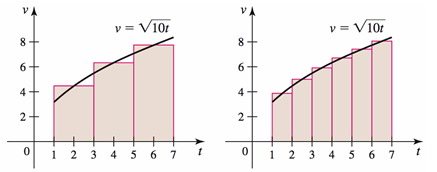
\includegraphics[scale=0.9]{Ch5Sect1_Exer10}
\end{center}
\end{frame}

% % %
\begin{frame}
\frametitle{\small Riemann Sums}
\small
%The more subintervals you divide your time interval into, the more accurate your approximation of displacement will be (see Example 1 on pp.\ 307--308).

%We now examine a method for approximating areas under curves.

Consider a function $f$ over the interval $[a,b]$.  Divide $[a,b]$ into $n$ subintervals of equal length:
\[[x_0,x_1], [x_1,x_2], \dots, [x_{n-1},x_n]\]
with $x_0=a$ and $x_n=b$.  The length of each subinterval is denoted
\[\Delta x = \frac{b-a}{n}.\]
\end{frame}

% % %
\begin{frame}
\small
In each subinterval $[x_{k-1}, x_k]$, we can choose any point $\overline{x}_k$ and create a rectangle with a height of $f(\overline{x}_k)$.
The area of the rectangle is the product of its height and base, or $f(\overline{x}_k)\Delta x$.

\vspace{1pc}
Doing this for each subinterval, and then summing each rectangle's area, produces an approximation of the overall area.  This approximation is called a {\bf Riemann sum}
\[R=f(\overline{x}_1)\Delta x + f(\overline{x}_2)\Delta x + \cdots + f(\overline{x}_n)\Delta x.\]
\end{frame}

% % %
\begin{frame}
\footnotesize
Note:  We let $k$ vary from $1$ to $n$, and we always have 
\[x_{k-1}\leq \overline x_k\leq x_k.\]  
We usually choose $\overline{x}_k$ so that it is consistent across all the subintervals.  The most common ways to do this are with {\bf left Riemann sums}, {\bf right Riemann sums}, and {\bf midpoint Riemann sums}.  (See Figures 5.9--5.11 on pp.\ 310--312 for pictures of these sums.)

\vspace{1pc}
Let $R=f(\overline{x}_1)\Delta x + f(\overline{x}_2)\Delta x + \cdots + f(\overline{x}_n)\Delta x$.
\begin{itemize}
\item[1.] $R$ is a {\bf left Riemann sum} when we choose $\overline x_k=x_{k-1}$ for each $k$.  
\item[2.] $R$ is a {\bf right Riemann sum} when we choose $\overline x_k=x_k$ for each $k$.
\item[3.] $R$ is a {\bf midpoint Riemann sum} when we take $\overline x_k$ to be the midpoint between $x_{k-1}$ and $x_k$, for each $k$.  
\end{itemize}
\end{frame}

% % %
\begin{frame}
\frametitle{\small Sigma Notation}
\footnotesize
Riemann sums become more accurate when we make $n$ (the number of rectangles) bigger.  However, writing it down becomes a pain.  Sigma notation gives a shorthand.  

%Recall how sigma notation works:  $\displaystyle\sum_{n=1}^5 n^2$ means to sum all integer values from the lowest limit ($n=1$) to the highest limit ($n=5$) in the summand $n^2$.  So 
\begin{ex} \[\dsum_{n=1}^5 n^2 = 1^2+2^2+3^2+4^2+5^2=55.\] \end{ex}

\begin{exe} Evaluate $\displaystyle\sum_{k=0}^3 (2k-1)$. \end{exe}
\end{frame}

% % %
\begin{frame}
\frametitle{\small $\Sigma$-Shortcuts}
\footnotesize
($n$ is always a positive integer)
\begin{align*}
\dsum_{k=1}^n c & = cn \text{ (where $c$ is a constant)} \\[0.5pc]
\dsum_{k=1}^n k &= \dfrac{n(n+1)}{2} \\[0.5pc]
\dsum_{k=1}^n k^2 &= \dfrac{n(n+1)(2n+1)}{6} \\[0.5pc]
\dsum_{k=1}^n k^3 &= \dfrac{n^2(n+1)^2}{4}
\end{align*}
\end{frame}

% % %
\begin{frame}
\frametitle{\small Riemann Sums Using Sigma Notation}
\small
Now using sigma notation, we can write the Riemann sum in a much more compact form:
\begin{align*}
R &= f(\overline{x}_1)\Delta x + f(\overline{x}_2)\Delta x + \cdots + f(\overline{x}_n)\Delta x \\[0.5pc]
 &= \dsum_{k=1}^n f(\overline{x}_k) \Delta x.
 \end{align*}

%To write the left, right, and midpoint Riemann sums in sigma notation, we need to know the point $\overline{x}_k$.
\end{frame}

% % %
\begin{frame}
\frametitle{\small Left, Right, and Midpoint Riemann Sums in Sigma Notation}
\footnotesize
Suppose $f$ is defined on a closed interval $[a,b]$ which is divided into $n$ subintervals of equal length $\Delta x$.  As before, let $\overline{x}_k$ denote a point in the $k$th subinterval $[x_{k-1},x_k]$, for $k=1,2,\dots,n$.  Also, notice that $x_0=a$ and $x_n=b$. 

\begin{itemize}
\item[1.] $\dsum_{k=1}^n f(\alert{a+(k-1)\Delta x}) \Delta x$ gives a left Riemann sum.
\item[2.] $\dsum_{k=1}^n f(\alert{a+k\Delta x}) \Delta x$ gives a right Riemann sum.
\item[3.] $\dsum_{k=1}^n f(\alert{a+\left(k-\dfrac{1}{2}\right)\Delta x}) \Delta x$ gives a midpoint Riemann sum.
\end{itemize}
\end{frame}

\begin{frame}%[t]
\frametitle{}
\begin{exe} Use sigma notation to write the left, right, and midpoint Riemann sums for the function $f(x)=x^2$ on the interval $[1,5]$ given that $n=4$.

\vspace{1pc}
Based on these approximations, estimate the area bounded by the graph of $f(x)$ over $[1,5]$.
\end{exe}
\end{frame}

% % %
\begin{frame}
\frametitle{HW from Section 5.1}
Do problems 9, 11, 15--23 odd, 31, 33, 53--57 all (pp.\ 315--320 in textbook)
\end{frame}

\begin{comment}
\end{comment}

\end{document}